\chapter{SYSTEM DESIGN}

\section{Project Design}
The project design phase translates the conceptual requirements into technical specifications. It follows a structured approach to define the architecture, data structures, and procedural details of the "CivicGuard" platform.

\section{System Architecture}
The CivicGuard system architecture is designed to be highly modular and scalable, utilizing the Laravel MVC framework. It connects users via a web browser to a central server that processes business logic and interacts with a persistent PostgreSQL database. The architecture is decoupled to ensure that frontend changes do not affect backend stability and vice versa.

\begin{figure}[H]
    \centering
    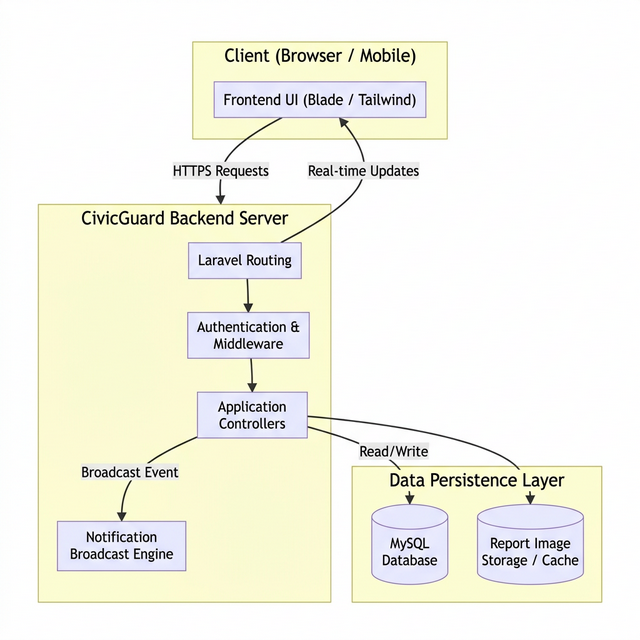
\includegraphics[width=0.9\textwidth]{images/system_architecture.png}
    \caption{System Architecture - Overview}
\end{figure}

The diagram above illustrates the multi-tier architecture, a standard for modern web platforms. The **Presentation Layer** (Blade/Tailwind) ensures that user inputs are captured through a responsive, low-latency interface. These inputs are then securely transmitted to the **Application Layer** (Laravel Controllers/Services), where complex business rules—such as image validation and departmental routing—are enforced. Finally, the **Data Layer** (PostgreSQL) provides a highly optimized relational storage environment. This tiered separation minimizes the impact of changes in any single layer, allowing the system to scale effectively as the user base grows.

Citizens initiate the lifecycle by registering and submitting reports. Officers interact with the system to process these reports and provide resolutions. Administrators act as the ultimate moderators, managing both users and system-wide configurations. This model ensures that all essential user stories are accounted for in the system logic.

\section{Activity Diagram}
The Activity diagram illustrates the dynamic flow of control within the report submission and resolution process. It focuses on the sequential and conditional steps taken from the moment a citizen logs in to the final resolution of a civic issue.

\begin{figure}[H]
    \centering
    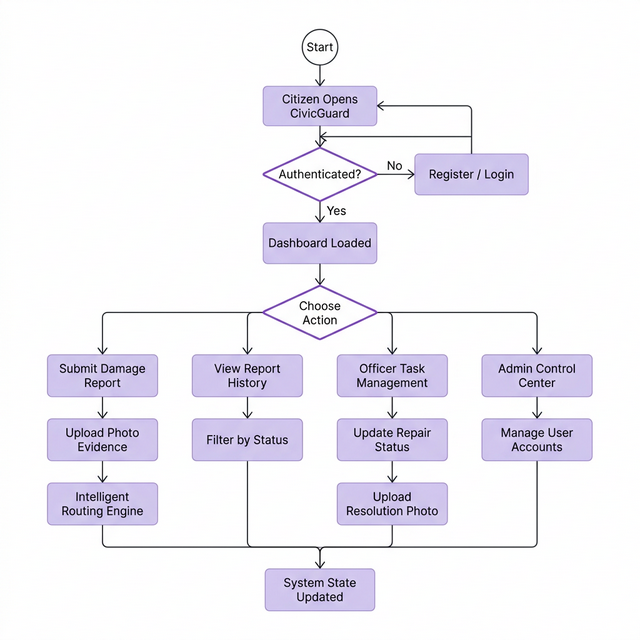
\includegraphics[width=0.8\textwidth]{images/activity_diagram.png}
    \caption{Activity Diagram - Report Lifecycle Control Flow}
\end{figure}

The flow begins with the **Citizen Authentication**, leading to a personalized dashboard where the **Submit Report** feature is prominent. A critical decision point in the logic is the **Evidence Upload**, which requires the system to handle binary data streams and local storage pathing. Once the input is validated against our strict business rules, the **Intelligent Routing Engine** asynchronously assigns the report to the appropriate department head. The activity lifecycle is only finalized when an officer physically inspects the damage, performs the repair, and uploads a "Resolution Photo," ensuring a closed-loop accountability system.

\section{Entity Relationship (ER) Diagram}
The database schema for CivicGuard is designed to maintain high integrity and relational consistency. It uses a normalized structure to minimize redundancy and optimize query performance.

\begin{figure}[H]
    \centering
    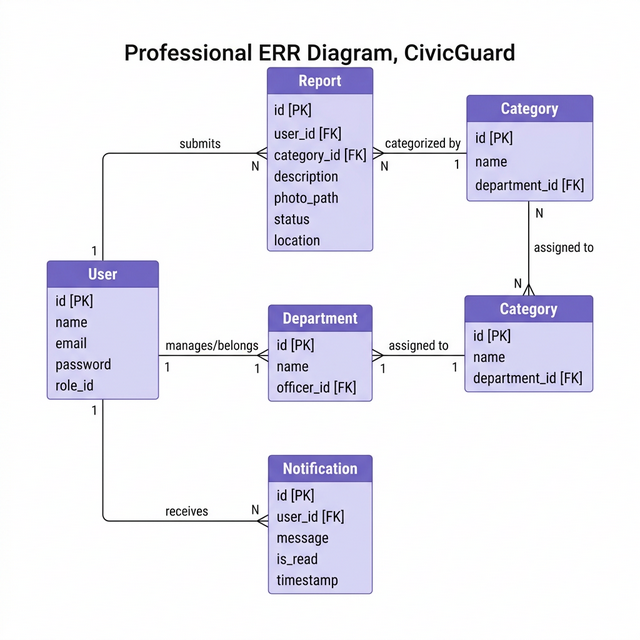
\includegraphics[width=0.8\textwidth]{images/er_diagram.png}
    \caption{ER Diagram - Database Schema}
\end{figure}

Key entities in our normalized schema include **Users**, **Reports**, **Departments**, and **Notifications**. The primary relationship is a one-to-many link between Users and Reports, reflecting the reality that a single active citizen may report multiple infrastructure issues over time. Furthermore, the mandatory link between a Report and a Department ensures that no "orphaned" reports exist in the system. Our schema also incorporates timestamping on every status change, allowing for the generation of "Mean-Time-To-Repair" (MTTR) analytics.

\section{Class Diagram}
The system architecture follows the MVC (Model-View-Controller) pattern, as demonstrated in the Class Diagram below. These classes represent the actual PHP code structure within the Laravel `app/` directory.

\begin{figure}[H]
    \centering
    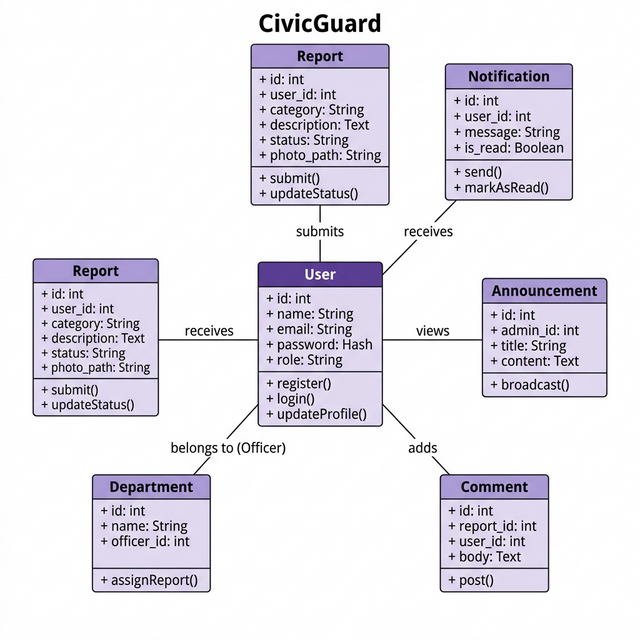
\includegraphics[width=0.8\textwidth]{images/class_diagram.png}
    \caption{Class Diagram - System Architecture}
\end{figure}

The diagram illustrates our core models (`User`, `Report`, `Notification`) and their tightly coupled controllers. The `ReportController` serves as the primary gateway, encapsulating the methods for both `store()` (citizen submission) and `update()` (officer resolution). We utilize a "Service Pattern" for the routing logic, ensuring that the controller remains lean and focused on HTTP orchestration. This clean partitioning of code into models (data), views (UI), and controllers (logic) makes the CivicGuard codebase exceptionally robust and easy to audit for security vulnerabilities.

\section{Sequence Diagram}
The sequence diagram details the chronological flow of report submission and status updates, focusing on the messages exchanged between objects over time.

\begin{figure}[H]
    \centering
    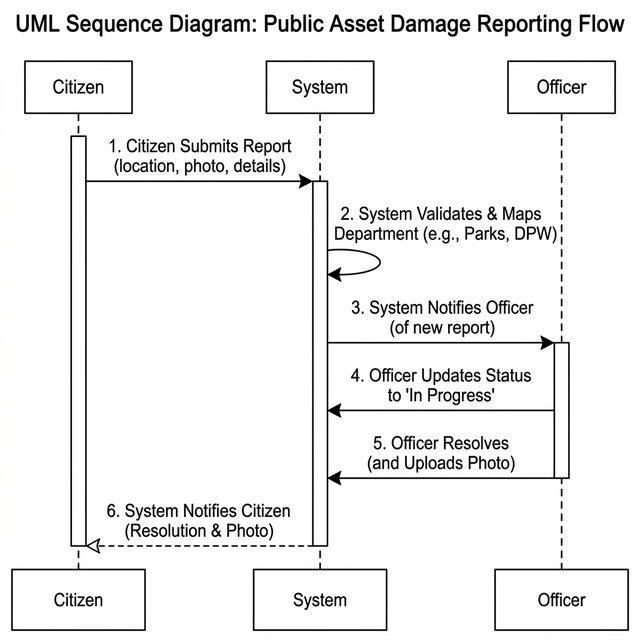
\includegraphics[width=0.8\textwidth]{images/sequence_diagram.png}
    \caption{Sequence Diagram - Report Lifecycle Message Flow}
\end{figure}

It shows the step-by-step interaction between the Citizen, the Laravel Backend, and the Department Officer. When a user submits a report, the backend validates the data, stores the image in the server's file system, and creates a database entry. A notification is then automatically pushed to the relevant officer's dashboard, completing the initial sequence.

\section{Project Pipeline}
The development and deployment pipeline for CivicGuard ensures continuous quality and smooth delivery, following a structured SDLC as illustrated in the figure below.

\begin{figure}[H]
    \centering
    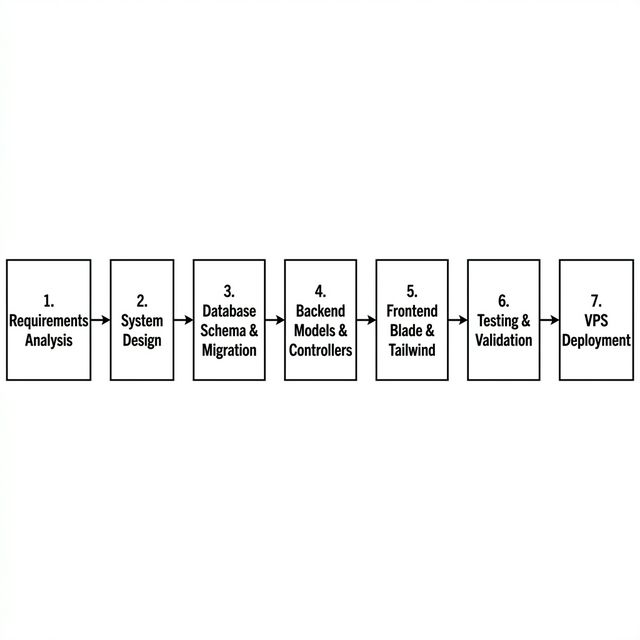
\includegraphics[width=0.95\textwidth]{images/project_pipeline_civicguard.png}
    \caption{Project Pipeline - Development Lifecycle}
\end{figure}

The pipeline covers everything from **Requirement Analysis** to **Final Deployment**. It includes specific stages for **Backend Development** using Laravel and **Quality Assurance** using professional testing tables. This disciplined approach minimizes bugs and ensures that the final product meets all user requirements.

\section{User Interface (UI) Design}
The User Interface (UI) design for CivicGuard adheres to modern usability standards, prioritizing clean layouts, accessibility, and a "premium" visual identity. It bridges the technical backend with a responsive, user-centric frontend.
The CivicGuard user interface is designed with a focus on modern aesthetic standards, ensuring that a technical tool remains accessible and "premium" in feel.

\begin{figure}[H]
    \centering
    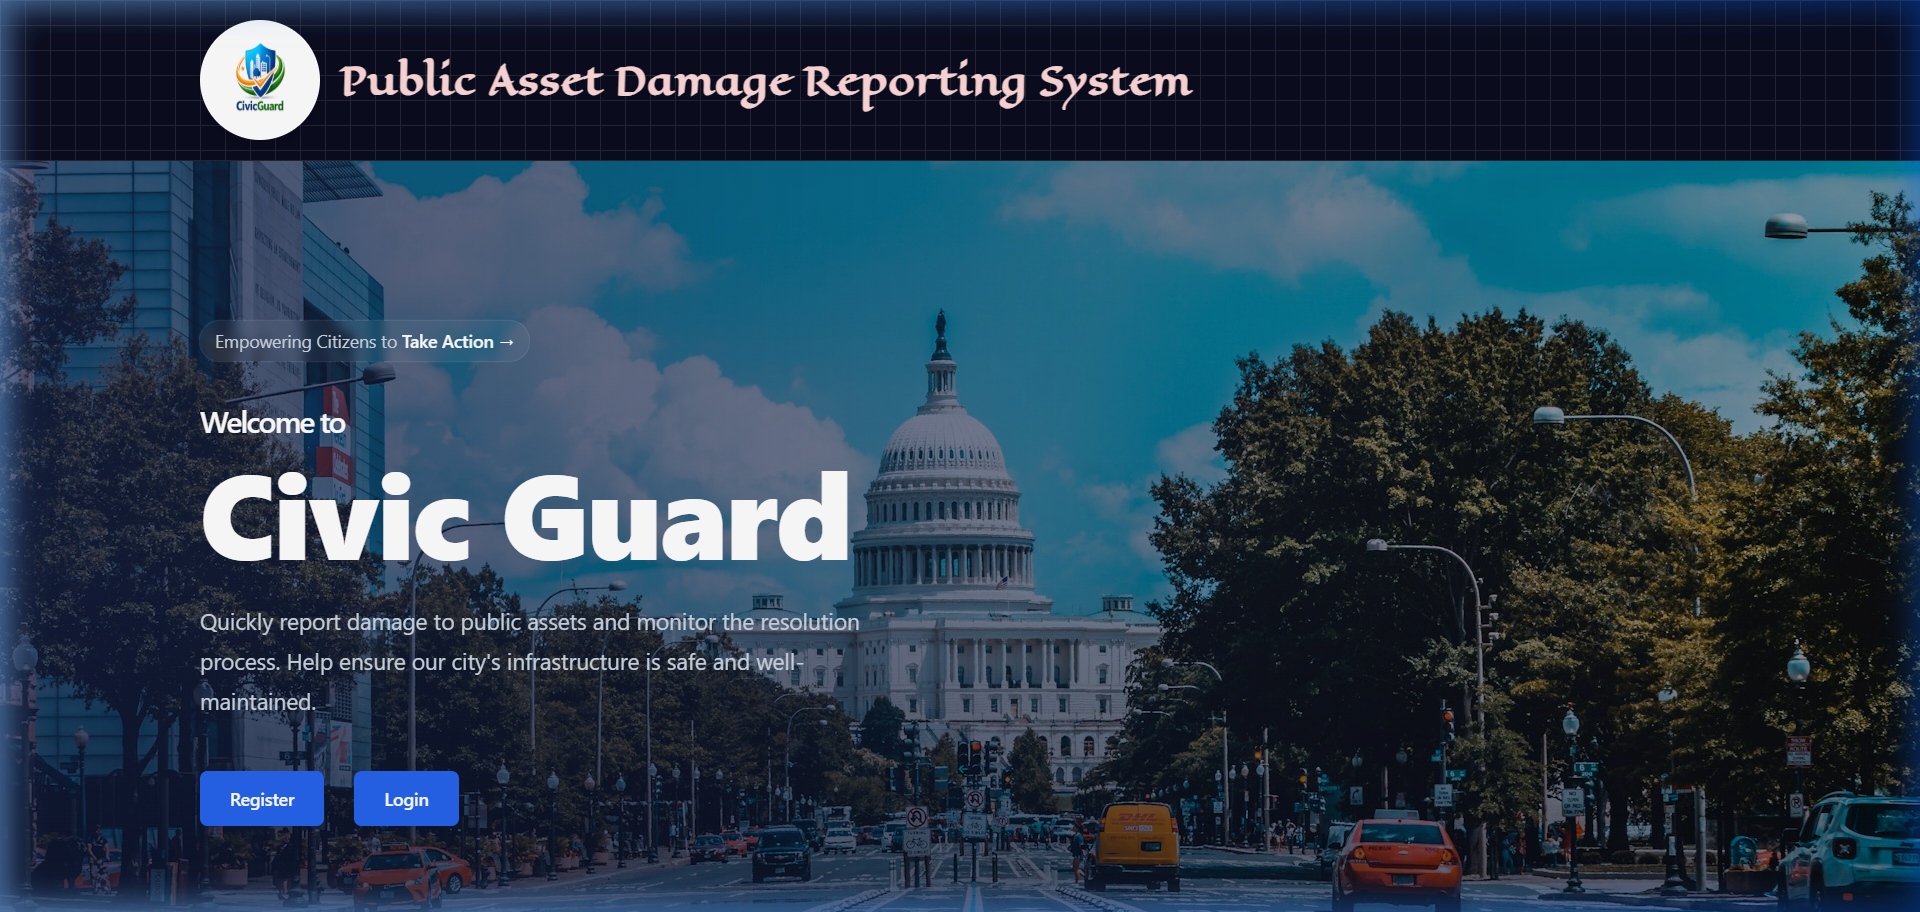
\includegraphics[width=0.8\textwidth]{images/landing_page.png}
    \caption{UI Design - Hero Section and Aesthetic Layout}
\end{figure}

The design follows a **Utility-First** approach using Tailwind CSS. Key principles include:
\begin{itemize}
    \item \textbf{Visual Hierarchy:} Using oversized typography and whitespace to guide the user's eye towards the "Report Now" button.
    \item \textbf{Status-Based Coloring:} Utilizing a curated palette (Amber for Pending, Emerald for Repaired) to provide instant visual feedback on report states.
    \item \textbf{Responsive Grid:} A mobile-first layout that ensures citizens can report issues comfortably from their smartphones while in the field.
\end{itemize}
